In the previous chapter a set of suggestions for improving a BPMN diagram where listed. As it was also mentioned, only a fraction of these improvements can be automated. 

This chapter will provide a example how the mentioned not automatable and automatable suggestions can be applied together to an existing BPMN model. 

\section{The example model}
The used BPMN model for this chapter will be a client registration process which is a real live process used in the telecommunication filed that was changed in order to be used in this thesis. The process model can be found in figure \ref{fig:example-process}

\begin{figure}[H]
	\centering
	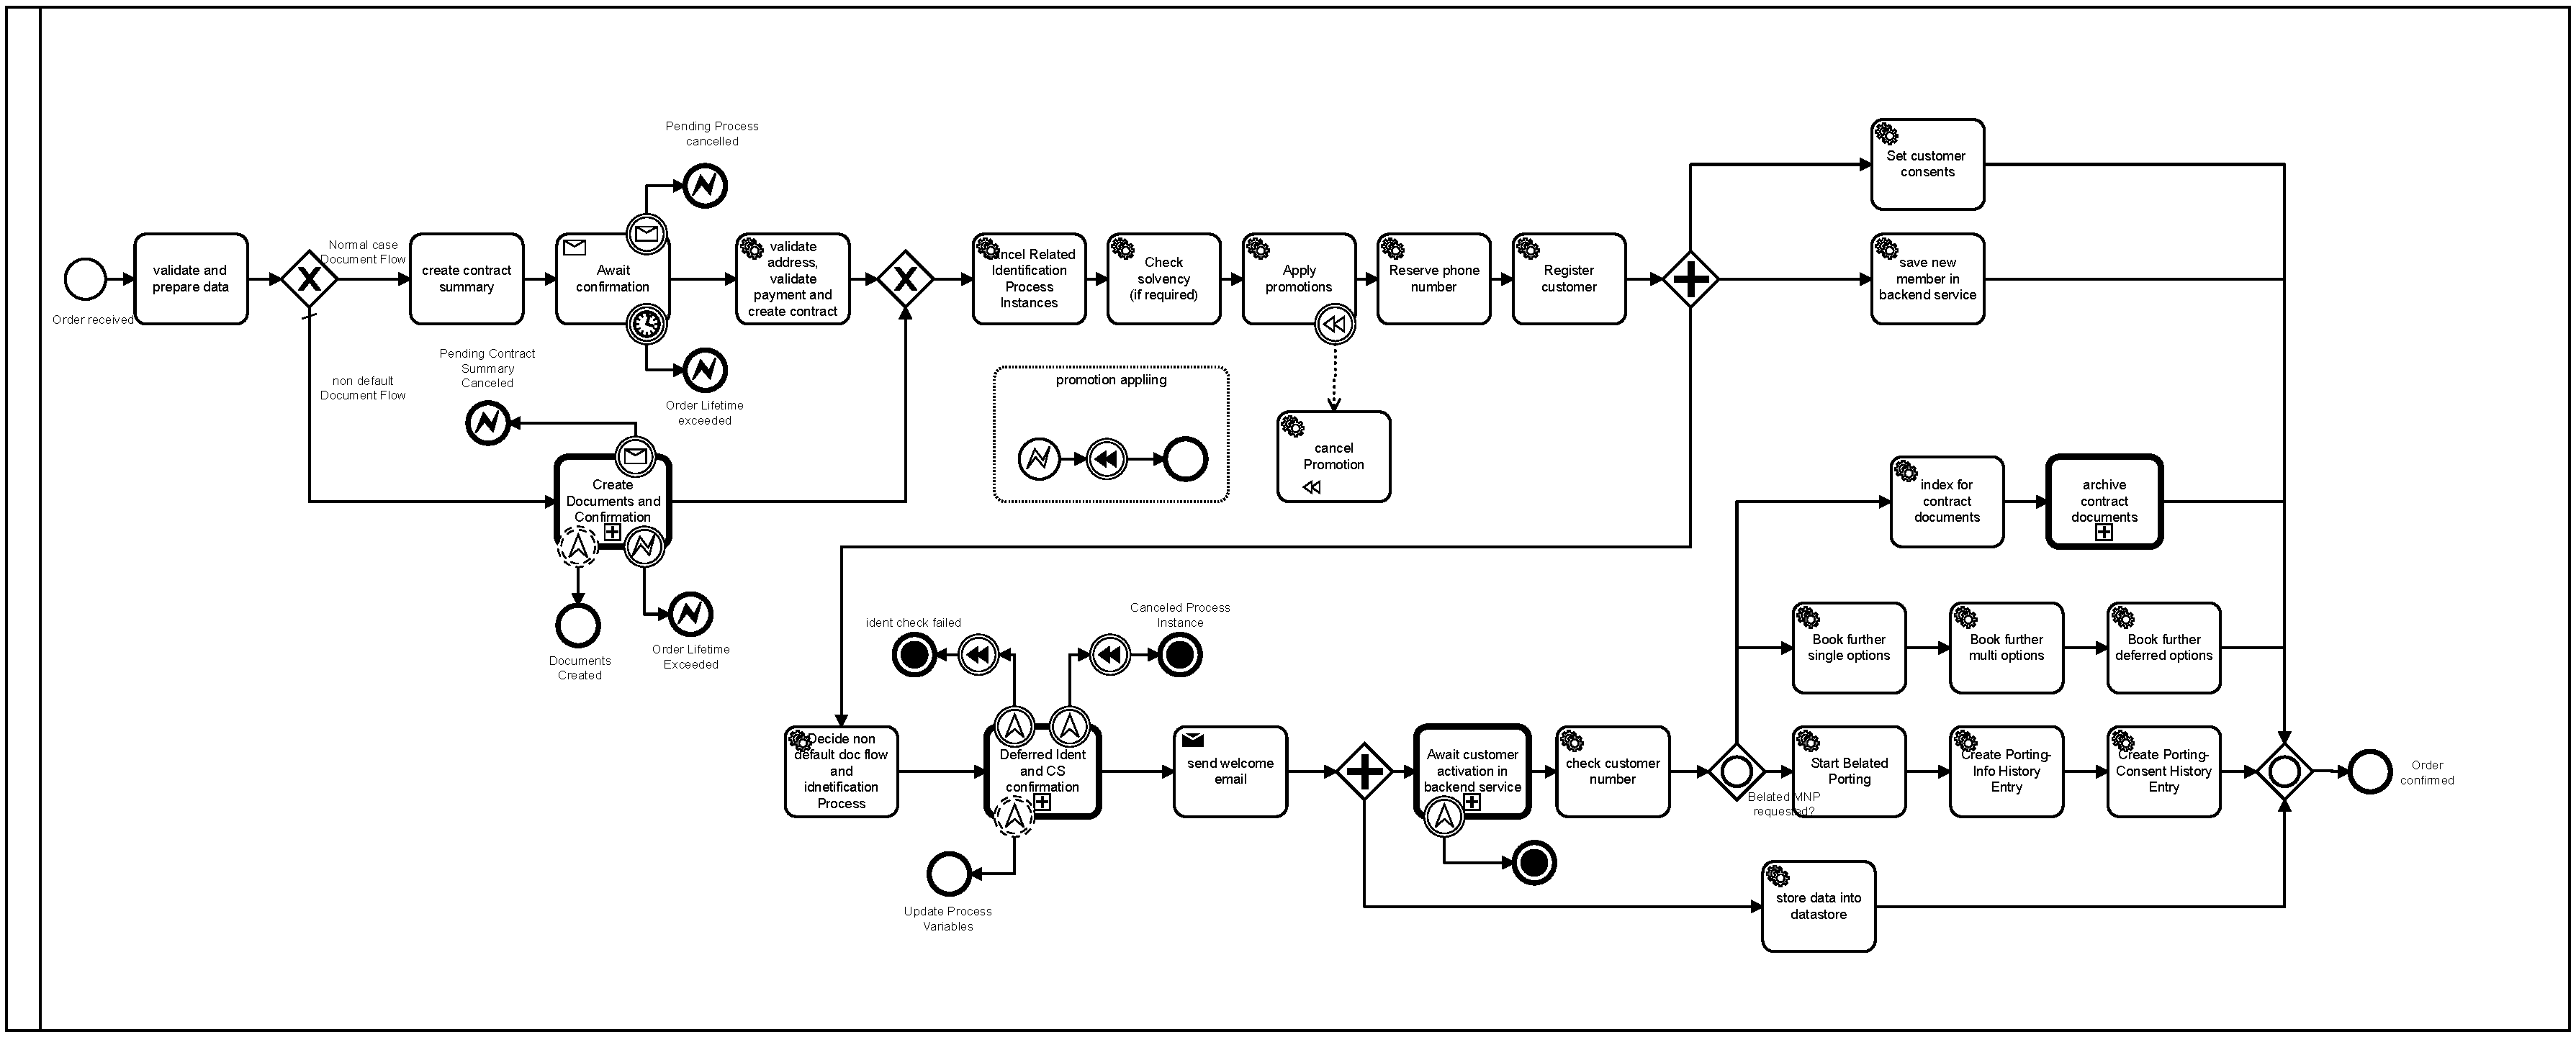
\includegraphics[width=1.7\columnwidth, angle=90 ]{graphics/process-bpmn.pdf}
	\caption{Example of a process where tasks can be merged together} 
	\label{fig:example-process} 
\end{figure}

\section{Evaluation by the Software}
\section{Comply with Naming Conventions}
%TODO
%see  https://docs.camunda.io/docs/components/best-practices/modeling/creating-readable-process-models/
%   & https://docs.camunda.io/docs/components/best-practices/modeling/naming-bpmn-elements/
\subsection{renaming tasks}
\subsection{renaming gateways}
\subsection{rename events}

\section{Extend automation boundaries}
%TODO

\section{Eliminate Manual Tasks}
%TODO

\section{Complete the process model}
%TODO

\section{No two consecutive Tasks handled by the same resource}
%TODO

\section{Inclusive Gateways over combining parallel and exclusive Gateways}
%TODO

\section{Value Added Analysis}
%TODO

\section{Evaluate Suggestions Quantitative}
%TODO

